% Created 2022-05-22 Sun 13:40
% Intended LaTeX compiler: xelatex
\documentclass[11pt]{article}
\usepackage{graphicx}
\usepackage{longtable}
\usepackage{wrapfig}
\usepackage{rotating}
\usepackage[normalem]{ulem}
\usepackage{amsmath}
\usepackage{amssymb}
\usepackage{capt-of}
\usepackage{hyperref}
\usepackage{color}
\usepackage{listings}
\usepackage[newfloat]{minted}
\usepackage[utf8]{inputenc}
\usepackage[table,xcdraw]{xcolor}
\usepackage{paralist}
\usepackage{datetime2}
\usepackage{graphicx}
\usepackage{lscape}
\usepackage{longtable}
\usepackage{hyperref}
\usepackage[a4paper, left=3cm, right=3cm, top=2cm]{geometry}
\usepackage{fancyhdr}
\usepackage{listings}
\usepackage{textcomp}
\usepackage{enumitem}
\usepackage{algorithm}
\usepackage{algpseudocode}
\setlist{noitemsep}
\setlength{\columnseprule}{0.2pt}
\definecolor{mygreen}{rgb}{0,0.6,0}
\definecolor{mygray}{rgb}{0.5,0.5,0.5}
\definecolor{mymauve}{rgb}{0.58,0,0.82}
\lstset{ backgroundcolor=\color{white}, basicstyle=\footnotesize, breaklines=true, captionpos=b, commentstyle=\color{mygreen}, escapeinside={\%*}{*)},keywordstyle=\color{blue}, stringstyle=\color{mymauve},}
\author{Olivier Lischer}
\date{\today}
\title{Design Patterns - Summary}
\hypersetup{
 pdfauthor={Olivier Lischer},
 pdftitle={Design Patterns - Summary},
 pdfkeywords={},
 pdfsubject={},
 pdfcreator={Emacs 27.2 (Org mode 9.5.2)}, 
 pdflang={English}}
\begin{document}

\pagestyle{fancy}
\fancyhf{}
\fancyhead[R]{SEP2-FS}
\fancyhead[L]{Design Patterns - Summary}
\fancyfoot[CE,CO]{\leftmark}
\fancyfoot[R]{\thepage}
\fancyfoot[L]{Olivier Lischer}

\begin{titlepage}
  \begin{center}
    {\Huge Design Patterns - Summary} \\
    \vspace{8 cm}

    
\includegraphics[height=4cm]{./img/ost-logo.png}

    \vspace{4 cm}
    Semester: Spring 2022
    \vspace{1 cm}

    Version: 0.1.0 \\
    Date: \DTMnow \\
    \vspace{3 cm}
    School of Computer Science\\
    OST Eastern Switzerland University of Applied Sciences
  \end{center}
\end{titlepage}
\newpage
\tableofcontents
\newpage


\section{Introduction}
\label{sec:org1f92b24}
\subsection{Most important quotes}
\label{sec:org9fe9ffe}
In the introduction the basics of object-oriented programming are explained.
Therefore, for many this is easy to read.
However, some important statements are made.

\begin{quote}
Favor object composition over class inheritance
\end{quote}

Because it is very difficult to make the correct abstraction often the base class(es) are not complete or have too much in it.
With object composition you don't have this problem.

\begin{quote}
Program to an interface, not an implementation
\end{quote}
If you implement against interfaces you can test your class with unit tests.
If you implement against a fixed implementation you can not change this behavior at anytime.

\subsection{The design patterns}
\label{sec:orgdf3c563}

Class Design Patterns deal with the relationships between classes and their subclasses.
The Object Design Patterns with the object relationships which can be changed at runtime.

\begin{figure}[htbp]
\centering
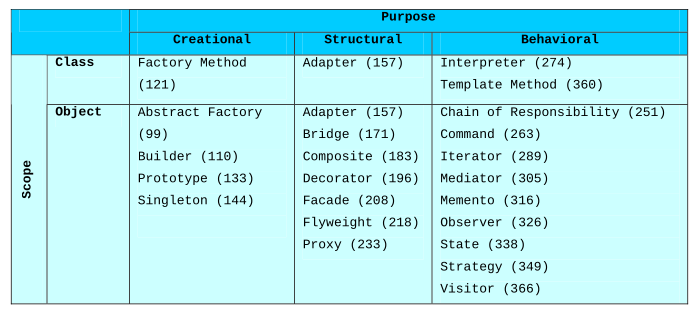
\includegraphics[width=.9\linewidth]{img/design_pattern_space.png}
\caption{\label{fig:design-pattern-space}Design pattern space}
\end{figure}


\section{Design Patterns}
\label{sec:org728c4a9}
\subsection{Creational}
\label{sec:orgd237e5b}
\subsubsection{Abstract Factory}
\label{sec:orgc45a845}
The Abstract Factory provides an interface for creating families of related or dependent objects without specifying their concrete class.
It is a good choice, when you want to create big class hierarchy from a factory.
In general the Simple Factory (\href{../../../../roam/20220510160458-design_pattern_simple_factory.org}{Design Pattern - Simple Factory}) is more common today.


Motivation:
\begin{itemize}
\item You want to create concrete objects without knowing which concrete type you get.
\item You are only interested in the interface.
\end{itemize}


\begin{figure}[htbp]
\centering
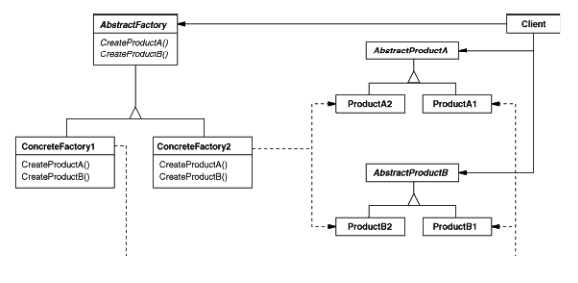
\includegraphics[width=.9\linewidth]{img/abstract_factory.png}
\caption{\label{fig:abstract-factory-uml}Abstract Factory Class Diagram}
\end{figure}

\begin{enumerate}
\item Important Notes
\label{sec:orgf608600}
The Factory must be created at the very beginning of the application.
After creation only this factory must be used to create objects.
Otherwise, the benefit of the factory are gone.
\end{enumerate}

\subsubsection{Builder}
\label{sec:org1178523}
The Builder Pattern seperates the construction of a complex class from its representation.
Therby you can hidde the creation of complex objects behind functions (see listening \ref{lst:the-builder-pattern-in-action}).


\begin{figure}[htbp]
\centering
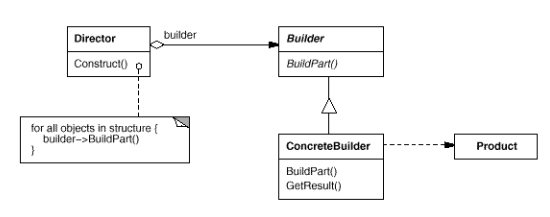
\includegraphics[width=.9\linewidth]{img/builder.png}
\caption{\label{fig:builder-class-diagram}Builder Class Diagram}
\end{figure}


\lstset{language=c++,label=lst:the-builder-pattern-in-action,caption={The Builder Pattern in Action},captionpos=b,numbers=none}
\begin{lstlisting}
Maze* MazeGame::CreateMaze () {
  Maze* aMaze = new Maze;
  Room* r1 = new Room(1);
  Room* r2 = new Room(2);
  Door* theDoor = new Door(r1, r2);
  aMaze->AddRoom(r1);
  aMaze->AddRoom(r2);
  r1->SetSide(North, new Wall);
  r1->SetSide(East, theDoor);
  r1->SetSide(South, new Wall);
  r1->SetSide(West, new Wall);
  r2->SetSide(North, new Wall);
  r2->SetSide(East, new Wall);
  r2->SetSide(South, new Wall);
  r2->SetSide(West, theDoor);
  return aMaze;
}

// With Builder Pattern
Maze* MazeGame::CreateMaze (MazeBuilder& builder) {
  builder.BuildMaze();
  builder.BuildRoom(1);
  builder.BuildRoom(2);
  builder.BuildDoor(1, 2);
  return builder.GetMaze();
}
\end{lstlisting}
\subsubsection{Factory Method}
\label{sec:org17ea09f}
The Factory Method is used to create an object, but the subclass decides which class is instantiated.
With this pattern you can create concrete creators which can decide which concrete product should be created.
The user of the creator only has to use the interface.


\begin{figure}[htbp]
\centering
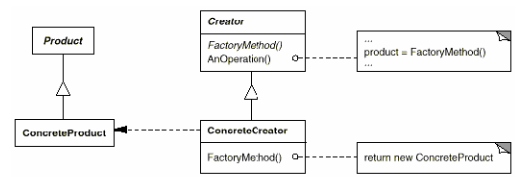
\includegraphics[width=.9\linewidth]{img/factory_method.png}
\caption{\label{fig:factory-method-class-diagram}Factory Method Class Diagram}
\end{figure}

\subsubsection{Prototype}
\label{sec:orga4ec4c7}
The prototype pattern is something similar like the factory method (\href{../../../../roam/20220413195351-design_pattern_factory_method.org}{Design Pattern - Factory Method}) is for classes.
Using the prototype pattern you create copies from concrete objects.
This is achieved by cloning the prototype.


\begin{enumerate}
\item Important Notes
\label{sec:orgc256503}
The crucial part of this pattern is the \texttt{Clone()} function.
During the implementation you have to decide if you want to do a deep copy or a shallow copy.


\begin{figure}[htbp]
\centering
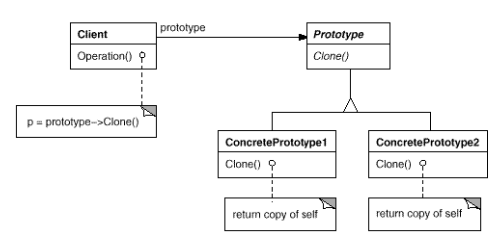
\includegraphics[width=.9\linewidth]{img/prototype.png}
\caption{\label{fig:prototype-class-diagram}Prototype Class Diagram}
\end{figure}


\lstset{language=c++,label=fig:prototype-design-patter-in-action,caption={Prototype Design Patter in Action},captionpos=b,numbers=none}
\begin{lstlisting}
class MazePrototypeFactory : public MazeFactory {
public:
  MazePrototypeFactory(Maze*, Wall*, Room*, Door*);
  virtual Maze* MakeMaze() const;
  virtual Room* MakeRoom(int) const;
  virtual Wall* MakeWall() const;
  virtual Door* MakeDoor(Room*, Room*) const;
private:
  vMaze* _prototypeMaze;
  Room* _prototypeRoom;
  Wall* _prototypeWall;
  Door* _prototypeDoor;
};

MazePrototypeFactory::MazePrototypeFactory (Maze* m, Wall* w, Room* r, Door* d) {
  _prototypeMaze = m;
  _prototypeWall = w;
  _prototypeRoom = r;
  _prototypeDoor = d;
}

Maze MazePrototypeFactory::MakeMaze () {
  return this->_prototypeMaze;
}
\end{lstlisting}
\end{enumerate}

\subsubsection{Singleton}
\label{sec:orga47f891}
The Singleton pattern ensures that a class has only one (global) instance.
Additionally, it provides easy access to this element.

However, you should \textbf{NOT} use it in your software.
It is basically a global variable.
Therefore, not testable and difficult to maintain.

If you want something like singleton, you should use a simple factory (\href{../../../../roam/20220510160458-design_pattern_simple_factory.org}{Design Pattern - Simple Factory}) which always returns the same instance.


\lstset{language=csharp,label=lst:singelton-alternative-in-code,caption={Singelton alternative in code},captionpos=b,numbers=none}
\begin{lstlisting}
class SingletonFactory {
    private static object myInstance;

    createObject() {
	if (SingletonFactory.myInstance == null) {
	    SingletonFactory.myInstance = new();
	}
	return SingletonFactory.myInstance;
    }
}
\end{lstlisting}

\begin{figure}[htbp]
\centering
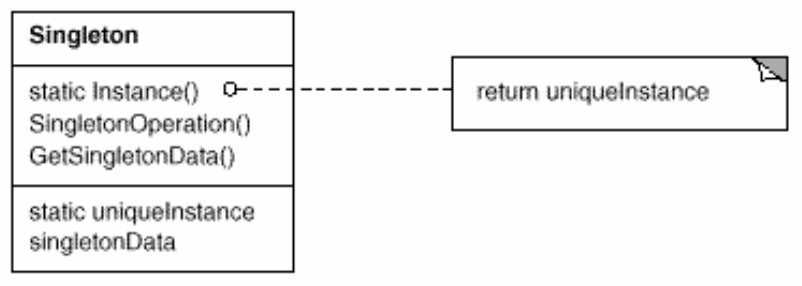
\includegraphics[width=.9\linewidth]{img/singleton.png}
\caption{\label{fig:singelton-class-diagram}Singelton Class Diagram}
\end{figure}

\subsection{Structural Patterns}
\label{sec:orgbbabb8d}
\subsubsection{Adapter}
\label{sec:org7ce6645}
The Adapter Design Pattern is used to make a class compatible to others (like a power adapter).
The adapter pattern has two different types:
\begin{itemize}
\item class adapter
\item object adapter
\end{itemize}


Both patterns do the same thing.
The class adapter inherits from the target \textbf{AND} from the adaptee (\ref{fig:class-adapter-class-diagram}).
The object adapter inherits only from the target and holds the adaptee as an instance variable (\ref{fig:object-adapter-class-diagram}).

The class adapter is not often used because many languages do not support multi-inheritance, and you should favor object composition over class inheritance.

\begin{figure}[htbp]
\centering
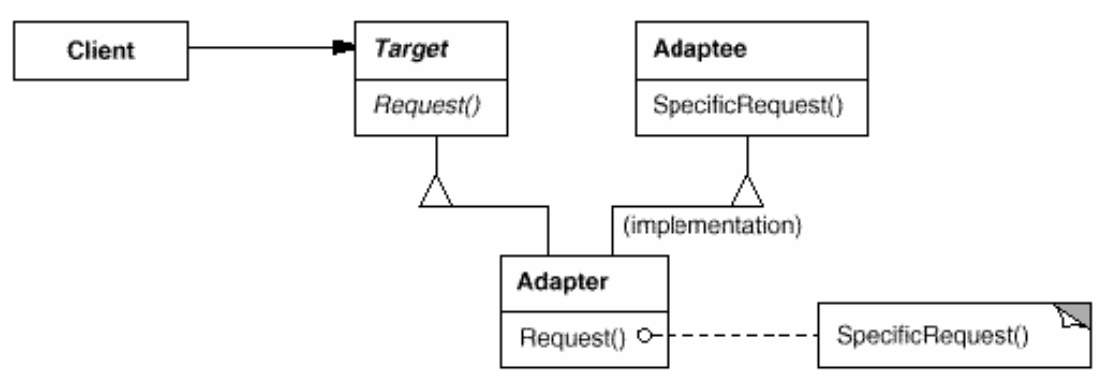
\includegraphics[width=.9\linewidth]{img/class_adapter.png}
\caption{\label{fig:class-adapter-class-diagram}Class Adapter Class Diagram}
\end{figure}

\begin{figure}[htbp]
\centering
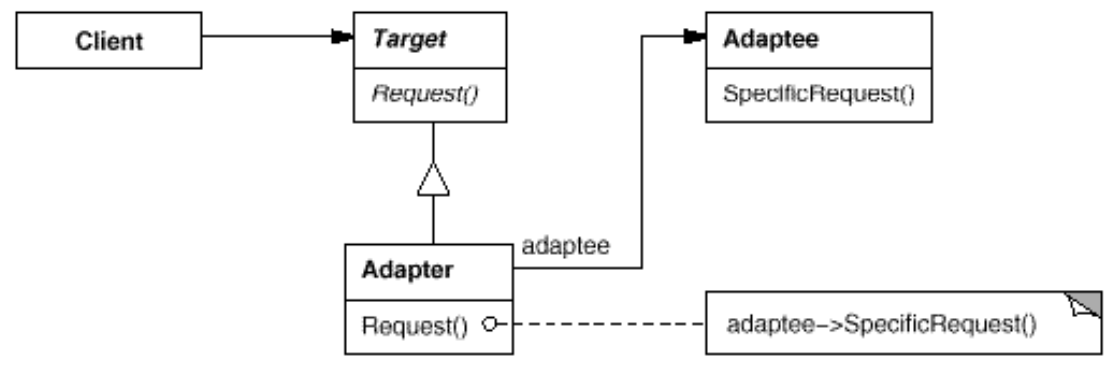
\includegraphics[width=.9\linewidth]{img/object_adapter.png}
\caption{\label{fig:object-adapter-class-diagram}Object Adapter Class Diagram}
\end{figure}
\subsubsection{Bridge}
\label{sec:org93a7ab0}
The Bridge Design Pattern is used to decouple an abstraction from its implementation so that the two can vary independently.

\begin{enumerate}
\item Example
\label{sec:orge64318a}
Your application should support multiple window systems (X, Windows).
The client (your application) should be able to create windows, without committing to a concrete implementation.
Only your window implementation should depend on the target platform (X, Windows).

\begin{figure}[htbp]
\centering
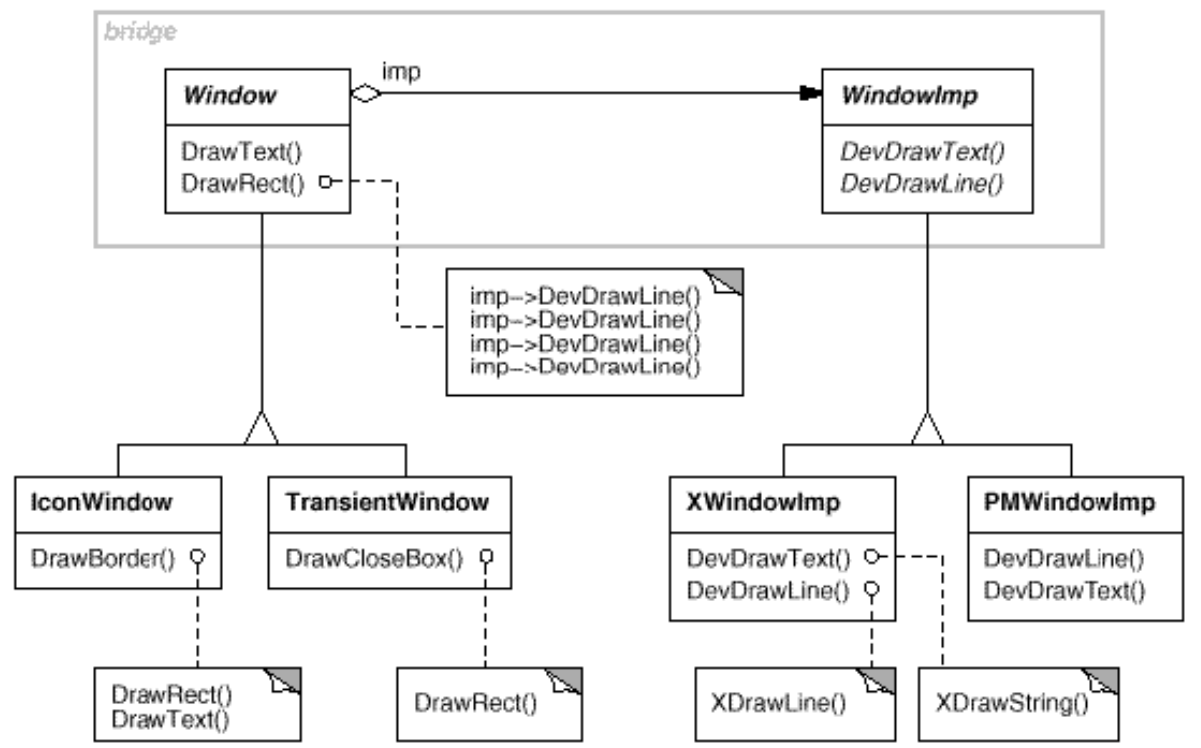
\includegraphics[width=.9\linewidth]{img/bridge_example.png}
\caption{\label{fig:bridge-design-pattern-example}Bridge Design Pattern Example}
\end{figure}

\begin{figure}[htbp]
\centering
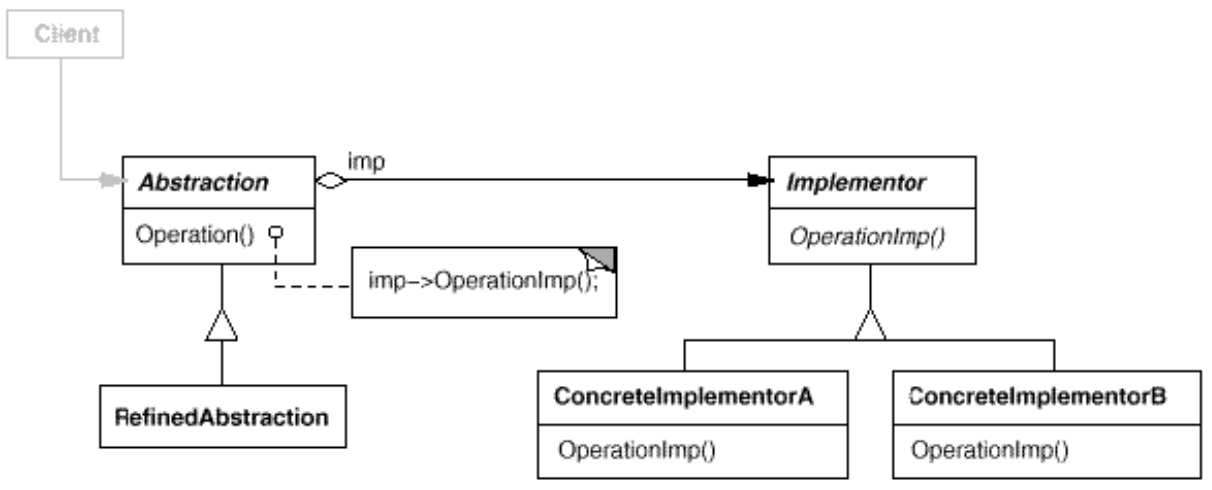
\includegraphics[width=.9\linewidth]{img/bridge.png}
\caption{\label{fig:bridge-class-diagram}Bridge Class Diagram}
\end{figure}
\end{enumerate}

\subsubsection{Composite}
\label{sec:orgec9083e}
The Composite Design Pattern is used to model a part-whole hierarchy.
The pattern let clients treat individual and compositions of objects uniformly.

\begin{figure}[htbp]
\centering
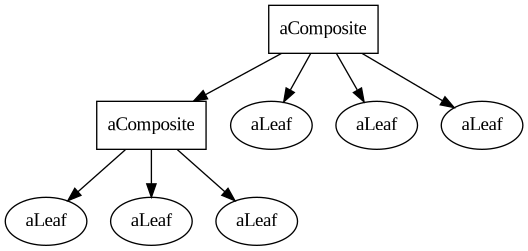
\includegraphics[width=.9\linewidth]{img/compsite_graph.png}
\caption{\label{fig:a-composite-structure}A Composite Structure}
\end{figure}


\begin{figure}[htbp]
\centering
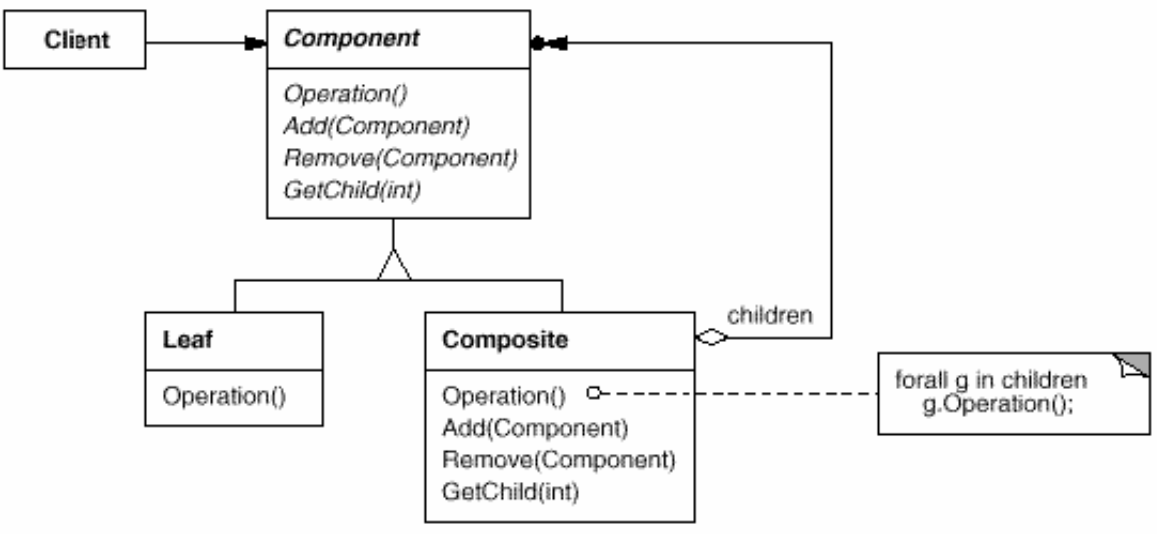
\includegraphics[width=.9\linewidth]{img/composite.png}
\caption{\label{fig:composite-diagram}Composite Diagram}
\end{figure}


\begin{enumerate}
\item Example
\label{sec:org4dfe066}
It exists many kinds of graphics and forms (Line, Rectangle, Picture, \ldots{}).
If the client wants to draw any graphic, it does not care how draw.
Therefore, we need one function (\texttt{draw}) for all kind of graphics.
However, a picture consists of many lines, rectangles and more graphics.
This picture class has some more functions (\texttt{Add}, \texttt{Remove}, \texttt{GetChild}).
The \texttt{Draw} function iterates over all children and calls their \texttt{Draw} function.




\begin{figure}[htbp]
\centering
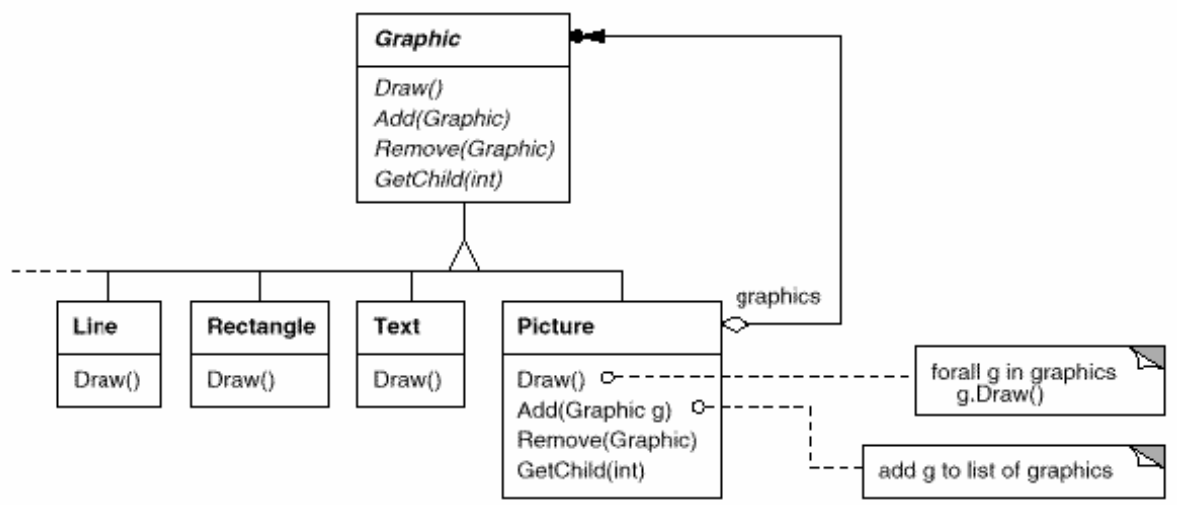
\includegraphics[width=.9\linewidth]{img/example_of_composite.png}
\caption{\label{fig:example-of-composite}Example of Composite}
\end{figure}
\end{enumerate}
\subsubsection{Decorator}
\label{sec:orgb6929a1}
The Decorater Pattern is used to attach additional responsibility (features) to an object dynamically.
For example, a class implements only the login mechanism.
Using the decorater pattern exception handling can be done in a separate class.


\begin{figure}[htbp]
\centering
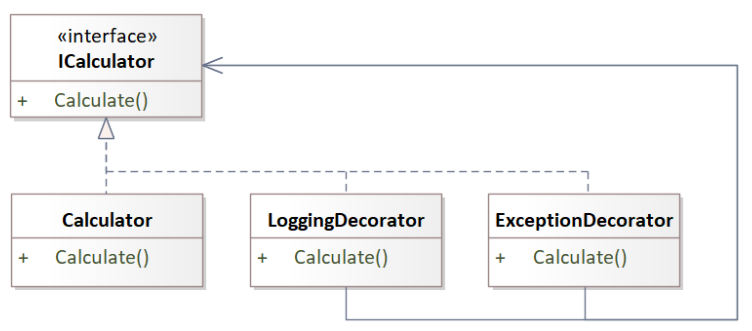
\includegraphics[width=.9\linewidth]{img/decorater.png}
\caption{\label{fig:decrater-diagram}Decrater Diagram}
\end{figure}


\subsubsection{Facade}
\label{sec:org7d96c0a}
The Facade Design Pattern is used to provide a simple interface to set of interfaces (subsystem).
For example the Compiler class provide an easy to use interface for the whole compiler subsystem (figure \ref{fig:facade-example}).


\begin{figure}[htbp]
\centering
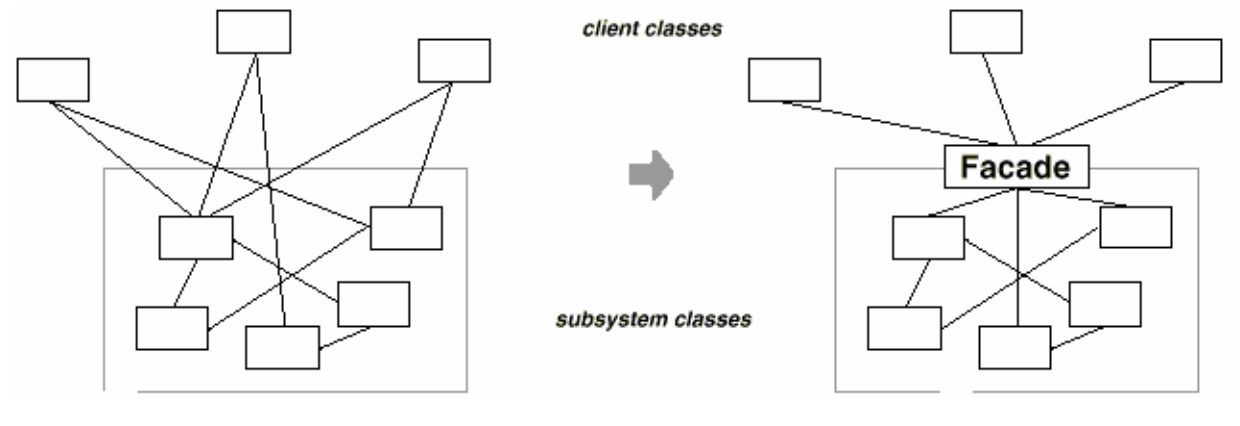
\includegraphics[width=.9\linewidth]{img/use_case_facade.png}
\caption{\label{fig:facade-use-case}Facade Use Case}
\end{figure}


\begin{figure}[htbp]
\centering
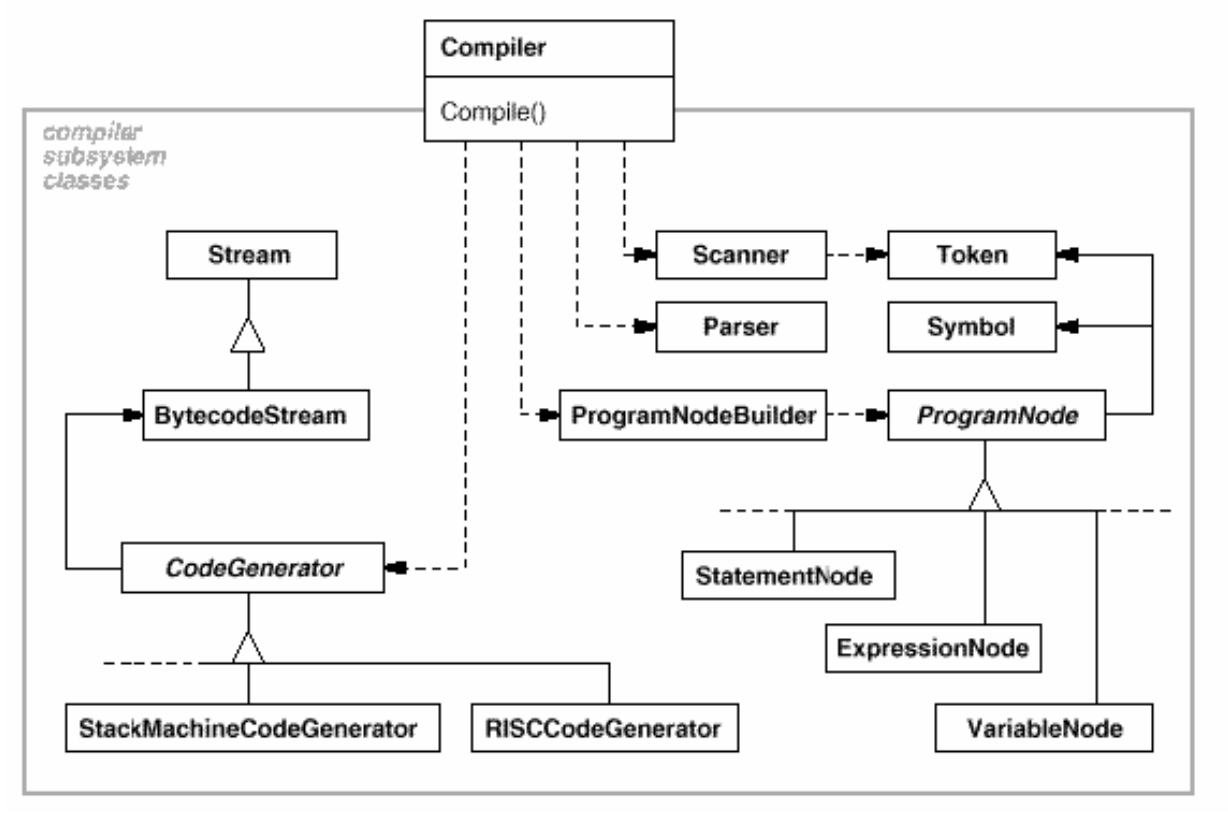
\includegraphics[width=.9\linewidth]{img/facade_example.png}
\caption{\label{fig:facade-example}Facade Example}
\end{figure}
\subsubsection{Flyweight}
\label{sec:org756e250}

The Proxy Design pattern provides a surrogate or placeholder for another object to control access to it.

A Feed Reader must load the news from a (slow) server.
When a frontend want to display the news before the data are availabel you have to provide a loading screen.
This can be easely done using the ProxyPattern.

The Proxy accepts the request, checks if the data are avaiable.
If not, it provides the login screen.
If the news are loaded, it returns the news.


\begin{figure}[htbp]
\centering
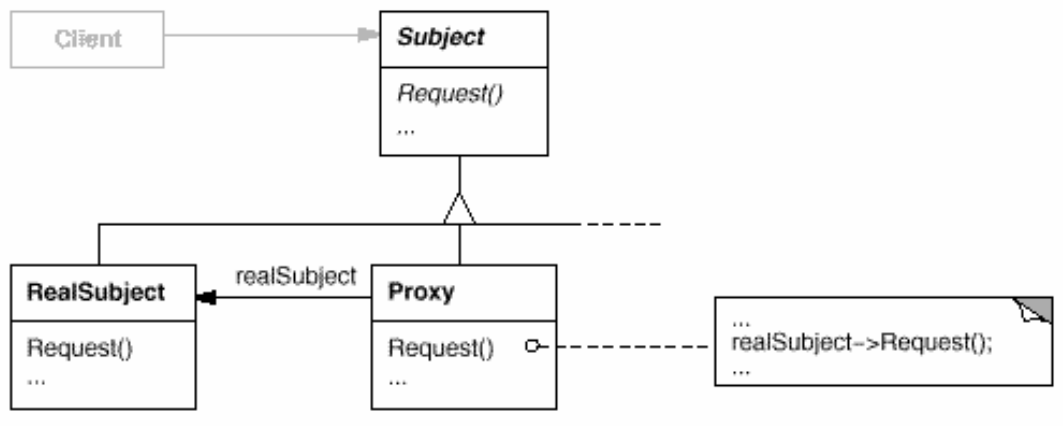
\includegraphics[width=.9\linewidth]{img/proxy.png}
\caption{\label{fig:proxy-class-diagram}Proxy Class Diagram}
\end{figure}


\begin{figure}[htbp]
\centering
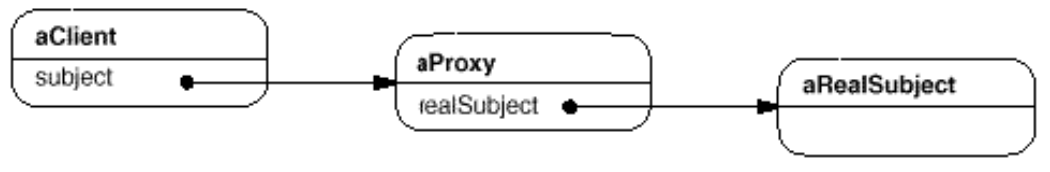
\includegraphics[width=.9\linewidth]{img/proxy_object_diagram.png}
\caption{\label{fig:object-diagram-for-proxy}Object Diagram for proxy}
\end{figure}
\subsubsection{Proxy}
\label{sec:org3c4a4d4}
The Proxy Design pattern provides a surrogate or placeholder for another object to control access to it.

A Feed Reader must load the news from a (slow) server.
When a frontend want to display the news before the data are availabel you have to provide a loading screen.
This can be easely done using the ProxyPattern.

The Proxy accepts the request, checks if the data are avaiable.
If not, it provides the login screen.
If the news are loaded, it returns the news.


\begin{figure}[htbp]
\centering
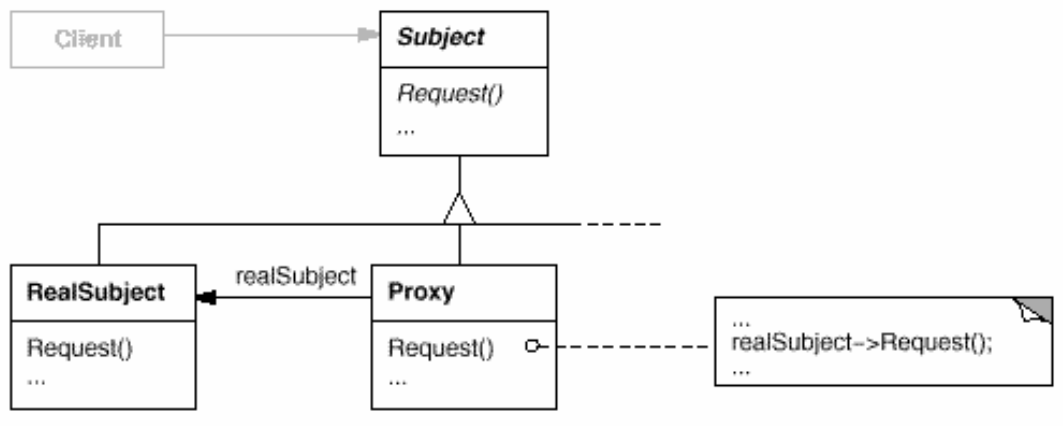
\includegraphics[width=.9\linewidth]{img/proxy.png}
\caption{\label{fig:proxy-class-diagram}Proxy Class Diagram}
\end{figure}


\begin{figure}[htbp]
\centering
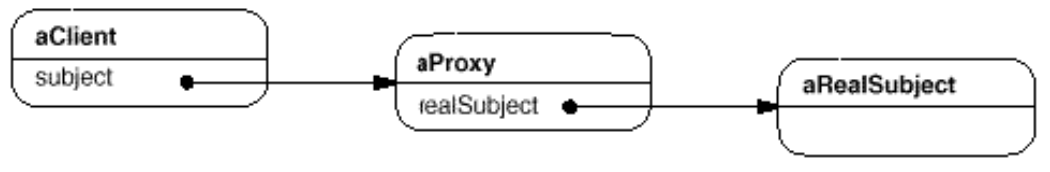
\includegraphics[width=.9\linewidth]{img/proxy_object_diagram.png}
\caption{\label{fig:object-diagram-for-proxy}Object Diagram for proxy}
\end{figure}
\end{document}